\documentclass{scrreprt}
\usepackage{listings}
\usepackage{array}
\usepackage{tikz} 
\usepackage{underscore}
\usepackage[bookmarks=true]{hyperref}
\usepackage[utf8]{inputenc}
\usepackage[english]{babel}
\usepackage{enumitem}
\usepackage[a4paper, margin=1in]{geometry}
\usetikzlibrary{shapes, arrows.meta, positioning, backgrounds}
\usetikzlibrary{arrows.meta}
\usetikzlibrary{shapes.geometric, positioning, arrows.meta}
\usetikzlibrary{positioning}
% Define styles for different node types
\tikzstyle{startstop} = [rectangle, rounded corners, minimum width=3cm, minimum height=1cm, text centered, draw=black, fill=red!30]
\tikzstyle{process} = [rectangle, minimum width=3.5cm, minimum height=1cm, text centered, draw=black, fill=blue!30]
\tikzstyle{arrow} = [thick,->,>=stealth]
% Define stickman style
\tikzset{
    startstop/.style={
        rectangle, rounded corners, minimum width=3cm, minimum height=1cm, text centered, draw=black, fill=gray!30
    },
    process/.style={
        rectangle, minimum width=3cm, minimum height=1cm, text centered, draw=black, fill=blue!30
    },
    decision/.style={
        diamond, aspect=2, minimum width=3cm, minimum height=1cm, text centered, draw=black, fill=orange!30
    },
    arrow/.style={
        thick, ->, >=stealth
    },
    stickman/.pic={
        % Head
        \draw[fill=gray] (0,0.6) circle (0.3cm);
        % Body
        \draw[line width=0.5mm] (0,0.3) -- (0,-0.6);
        % Arms
        \draw[line width=0.5mm] (-0.4,0.3) -- (0.4,0.3);
        % Legs
        \draw[line width=0.5mm] (0,-0.6) -- (-0.4,-1.2);
        \draw[line width=0.5mm] (0,-0.6) -- (0.4,-1.2);
}
}
\hypersetup{
    bookmarks=false,    % show bookmarks bar?
    pdftitle={Software Requirement Specification},    % title
    pdfauthor={Jean-Philippe Eisenbarth},                     % author
    pdfsubject={TeX and LaTeX},                        % subject of the document
    pdfkeywords={TeX, LaTeX, graphics, images}, % list of keywords
    colorlinks=true,       % false: boxed links; true: colored links
    linkcolor=blue,       % color of internal links
    citecolor=black,       % color of links to bibliography
    filecolor=black,        % color of file links
    urlcolor=purple,        % color of external links
    linktoc=page            % only page is linked
}
\usetikzlibrary{shapes, arrows.meta, positioning, backgrounds}

\tikzstyle{startstop} = [rectangle, rounded corners, minimum width=3cm, minimum height=1cm, text centered, draw=black, fill=red!30]
\tikzstyle{process} = [rectangle, minimum width=3.5cm, minimum height=1cm, text centered, draw=black, fill=blue!10]
\tikzstyle{database} = [rectangle, minimum width=3cm, minimum height=1cm, text centered, draw=black, fill=orange!30]
\tikzstyle{auth} = [rectangle, minimum width=3cm, minimum height=1cm, text centered, draw=black, fill=green!30]
\tikzstyle{ui} = [rectangle, minimum width=3.5cm, minimum height=1cm, text centered, draw=black, fill=yellow!30]
\tikzstyle{arrow} = [thick,->,>=stealth]



\usepackage{hyperref}
\begin{document}

\begin{titlepage}
    \centering
    \begin{center}
        
\includegraphics[width=0.5\textwidth]{logo.png} % Adjust width as necessary
    \end{center}
\begin{center}
    \textbf{Department of Computer Science and Engineering}\\
    Premier University
\end{center}
\begin{center}
    \textnormal{ CSE306: Software Engineering \& Information System Design Laboratory }
\end{center}
    \huge
    \textbf{Software Design Document}\\
    \vspace{0.5in}
    \LARGE
    \textbf{Odyssey Travel Agency Software}\\
    \vspace{1in}
    \large
    \textbf {Submitted by}\\
    \begin{center}
        \renewcommand{\arraystretch}{1.5} % Adjusts vertical spacing in the table
        \begin{tabular}{|>{\raggedright\arraybackslash}p{0.6\textwidth}|p{0.3\textwidth}|} % Adjust column widths
        \hline
        \textbf{Name} & \textbf{ID} \\
        \hline
        Mohammad Hafizur Rahman Sakib & 0222210005101118 \\
        \hline
        Arnab Shikder & 0222210005101098 \\
        \hline
        Mohammad Ohidul Alam & 0222210005101123 \\
        \hline
        Sayed Hossain & 0222210005101102 \\
        \hline
        Mohammad Asmual Hoque Yousha & 0222210005101121 \\
        \hline
        \end{tabular}
        \end{center}
    \vspace{0.5in}
 
\begin{minipage}[t]{0.5\textwidth}
        \textbf{Submitted to :}
        \\Jannatul Maowa Hasi
        \\Lecturer,Department of CSE
        \\ Premier University
        \\ Chittagong
    \end{minipage}%
    \begin{minipage}[t]{0.6\textwidth}
        \raggedleft
        \textbf{Remarks}\\
        \vspace{0.5cm} % Adjust vertical space for remarks
        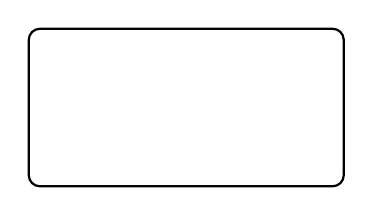
\begin{tikzpicture}
            \draw[thick, rounded corners] (0,0) rectangle (4,2);
        \end{tikzpicture}
    \end{minipage}

    \date{\today}
    \vfill
\end{titlepage}
\newpage
\end{document}
